% Chapter 1

\chapter{Application Architecture} % Main chapter title

\label{Chapter4} % For referencing the chapter elsewhere, use \ref{Chapter1} 

\lhead{Chapter 4. \emph{Application Architecture}} % This is for the header on each page - perhaps a shortened title

%----------------------------------------------------------------------------------------
The changing requirements caused architecure to change several times over the course of the project as components were first prototyped then tested. 

\section{Prototyping}

The initial prototypes included HelloWorld \footnote{HelloWorld is commonly a testbed to ensure the build environment and external libraries build correctly} application and simple game of BreakOut. HelloWorld and Breakout were both prototyped with the Cocos2d game engine because of the game engines ability to allow quick control over game objects. \cite{cocos2d} 

%later prototypes included

\subsection{HelloWorld}\label{HelloWorld_prototype}
The HelloWorld application tracked blocks across the screen using input data from the LeapMotion animating the interface. This application served as starting point for working with the LeapMotion SDK and also as a way of testing input received from the LeapMotion and resolving it to the coordinate space within the application. This code became a boiler plate interface to working with LeapMotion SDK later on in the project. 

\subsection{BreakOut}\label{breakout_prototype}
Furthering the HelloWorld application and testing the LeapMotion capabilities a simple game of BreakOut\footnote{The breakout game was pre-built sample code\cite{breakout}} was adapted for using the LeapMotion as the control mechanism for the paddle. This application was used in Session 2~\ref{session2} with the children to show sample interactions of a complete system. 

This prototype also showed through observation with the children how different methods of calculating the coordinates on the screen might be accomplished. The first method takes the position of the pointer in its coordinate space and translates it the coordinate space in the application as shown in Figure~\ref{fig:HandPosition} despite the orientation of the pointer. The second method uses a vector pointing from the tip of the pointer and finds where that vector intersects with the screen as seen in Figure~\ref{fig:PointerIntersect}. Between the two methods the second method of finding the intersection on the screen appeared to be most natural. 

\begin{figure}
\centering     %%% not \center
\subfigure[Left position]{\label{fig:a}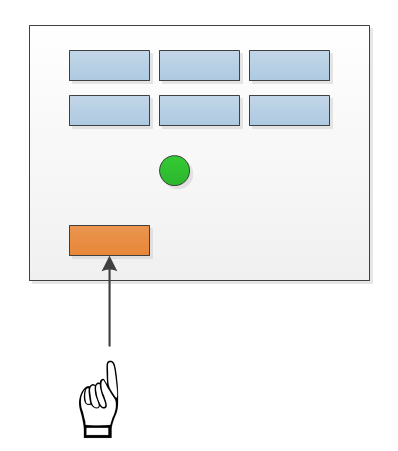
\includegraphics[width=60mm]{Pointer1}}
\subfigure[Right position]{\label{fig:b}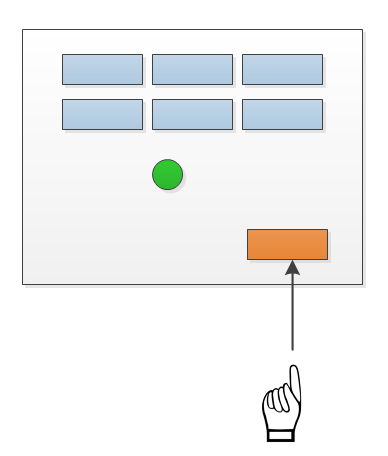
\includegraphics[width=60mm]{Pointer2}}
\caption{Left to right paddle control in breakout using the hand position relative to the screen }
\label{fig:HandPosition}
\end{figure}

\begin{figure}
\centering     %%% not \center
\subfigure[Left Position]{\label{fig:a}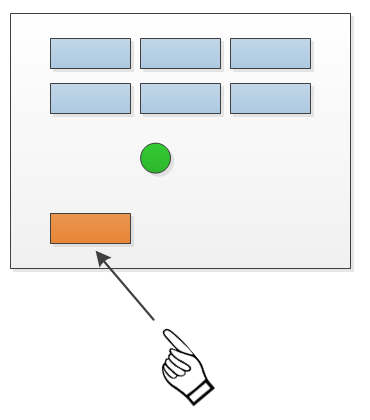
\includegraphics[width=60mm]{PointerIntersect1}}
\subfigure[Right position]{\label{fig:b}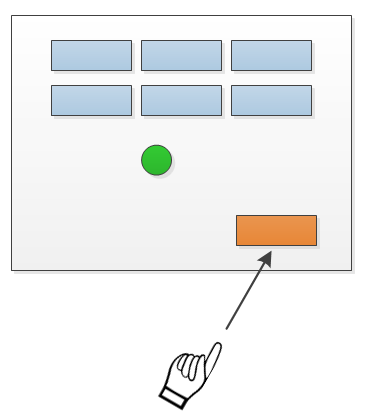
\includegraphics[width=60mm]{PointerIntersect2}}
\caption{Left to right paddle control in Breakout using the pointer intersection with the screen }
\label{fig:PointerIntersect}
\end{figure}

\subsection{Unity}\label{unity_prototype}
One of the main gestures in the requirements used fingers to indicate beginning and ending actions as part of the gesture. Attempting to model these gestures required a 3D environment that could show multiple pointer interactions with game objects which was not possible with Cocos2d. The LeapMotion SDK provided a API with Unity 3D Game Engine which could perform the modeling required to begin recognizing the gestures. It was through this prototype that it was found that the LeapMotion would not be able to detect fingers touching each other\footnote{A later released visualizer in the LeapMotion SDK would show the same resulut.}. \cite{unity}

\subsection{Quartz 2D}\label{quartz2d_prototype}

The Cocos2d engine is not designed particularly for drawing and rendering textures to images. Apples Quartz 2D and Cocoa libraries are well suited for this task providing a large array of built in functionalities. These libraries were used to create the prototype drawing application using some of the boilerplate code from the earlier Helloworld~\ref{HelloWorld_prototype} and Breakout~\ref{breakout_prototype} prototypes. The boilerplate code formed into a standard interface and coordinate system for working with the LeapMotion. \cite{appleapi}

%%TODO Name for this interface

This prototype worked well in testing in Session 4~\ref{session4} and was generally well recieved by childeren although they had one major requirement of adding a cursor in addition to some minor features. The cursor would show where the pointer was on the screen at any given time so they could position it prior to painting. The minor features included selecting brushes, erasing, changing the brush size, changing the brush type and opacity.  

\subsubsection{Challenges}
The cursor was very difficult to implement using the Quartz 2D and Cocoa because the libraries do not natively support layering and drawing simultaneously due to the way the rendering context functions as a single context. Creating independent views and transparent windows did not render correctly when attempting to simultaneously update each view. An alternative might be to put each functionality into separate applications running on different process threads although this was not possible because the LeapMotion can only be accessible from one process at a time. To create a cursor in  HUD layer the application needed to access the LeapMotion, HUD and Drawing objects simultaneously. This was the defining factor in returning to the Cocos2d Game Library because it support independent layering of views. \cite{appleapi}

\subsection{LeapPaint}\label{leappaint_prototype}

The prototype dubbed "LeapPaint" by the children consisted of a combination components from the earlier Helloworld~\ref{HelloWorld_prototype} and Breakout~\ref{breakout_prototype} prototypes managing input on a standard interface and output into different visible for drawing and the HUD. The layers were connected via a GameManager \footnote{GameManager takes the role of the ApplicationDelegate} passing the delegate actions between layers and interfaces. 

This prototype recieved the best reviews by the children in testing Session 6~\ref{session6} despite lacking some of the features of available in the Quartz 2D~\ref{quartz2d_prototype}. This architecture could be used going forward in adding features. 


\section{User Interface Layout}
The interface layout of controls was based upon a combination of designs made by the children as seen in Figure~\ref{fig:LeapPaintScreenshot} with the canvas to paint on centered and the user interface controls tucked to the sides of the canvas. 


\begin{figure}
\centering     %%% not \center
\subfigure[Mock Up]{\label{fig:a}\includegraphics[width=60mm]{Mockup}}
\subfigure[Screenshot]{\label{fig:b}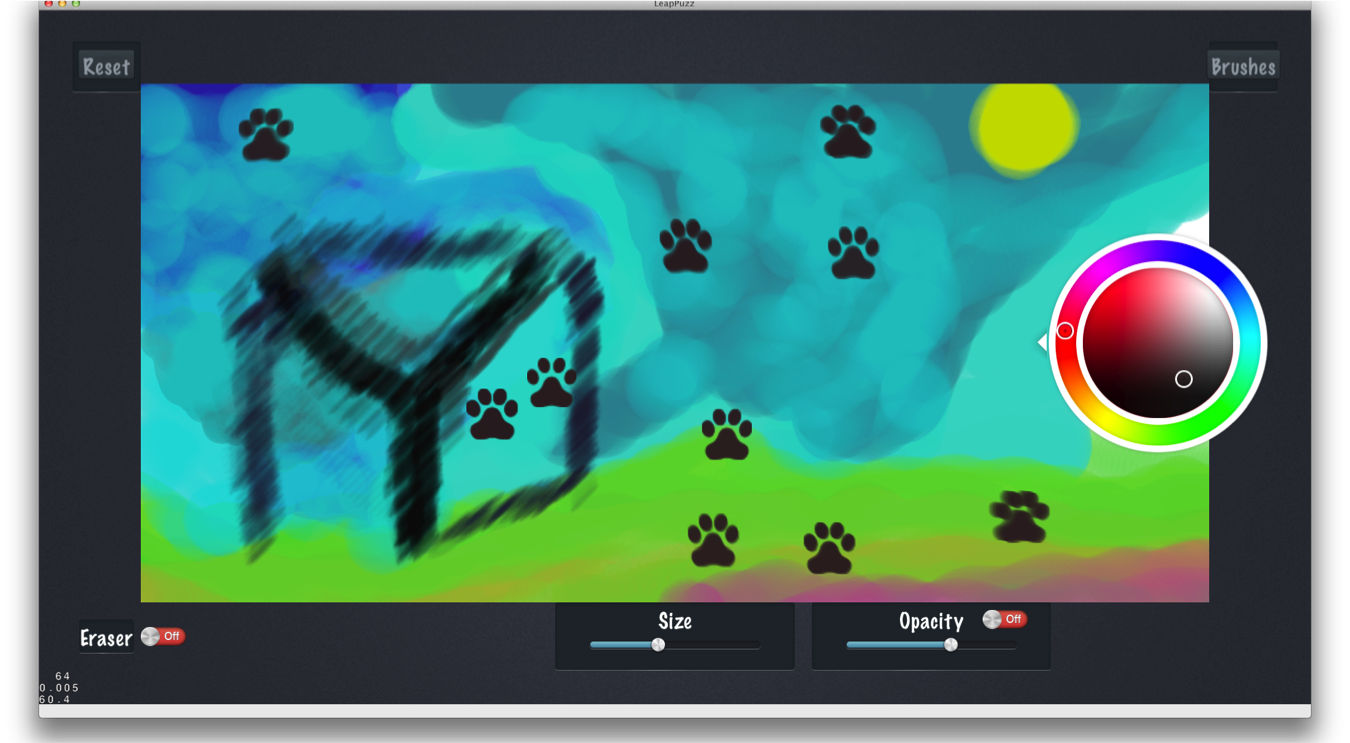
\includegraphics[width=60mm]{LeapPaintScreenshot}}
\caption{Mock up compared to a screen shot of finished application with a drawing. }
\label{fig:LeapPaintScreenshot}
\end{figure}



\subsection{pointer Tracking}
Initially a tracking system was design to use the relative coordinates of a pointer in the LeapMotion coordinate space and translate them to coordinates within the application. Later with the an SDK update the LeapMotion could provide coordinates on the screen where a vector from the pointers tip would intersect. This required some screen calibration to be performed such that the LeapMotion would be able to track points on the screen. 

\subsection{Application Layers}
The application was broken into component layers to manage and modularize different functionalities as seen in Figure~\ref{fig:applicationlayers}. This allowed for some components to become reusable for other applications by providing a common application programming interface (API). 

\begin{figure}
\centering
%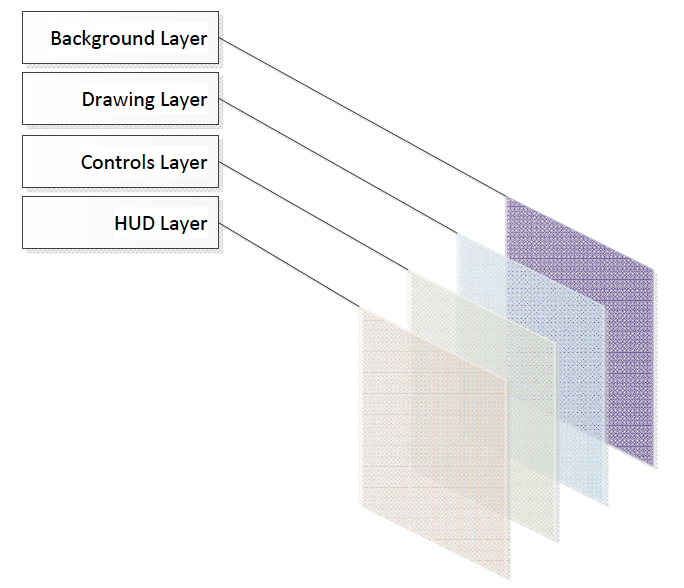
\epsfig{file=applicationlayers, height=0.65\columnwidth, width=\columnwidth}
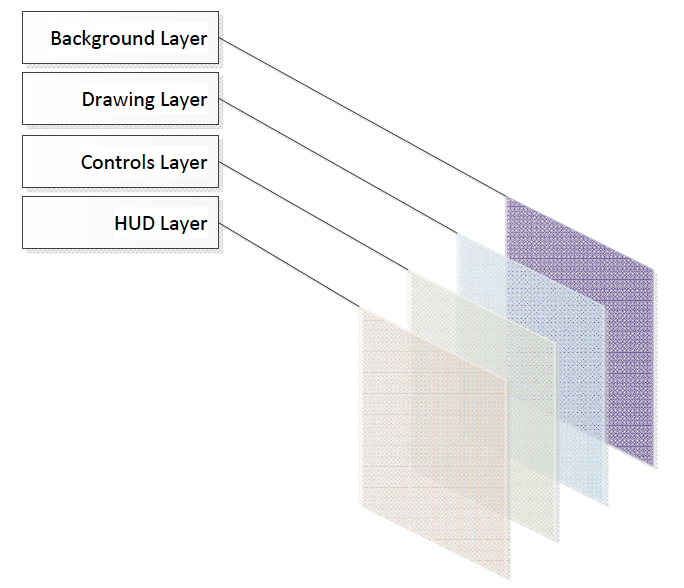
\includegraphics[height=0.65\columnwidth, width=\columnwidth]{applicationlayers}
\caption{The ordered layers of visibility in the application. }
\label{fig:applicationlayers}
\end{figure}

\begin{itemize}
\item Background Layer manages the background images and for the application. This practice is fairly standard and 
\item Drawing Layer is where the image will be edited and render. 
\item Controls Layer provides the user interface controls that for different aspects of the application.
\item HUD Layer displays feedback information for the position of the pointer in relation to the screen and any different actions that might be taking place. 
\end{itemize}

\section{External Libraries}

\begin{itemize}
\item LeapMotion SDK is the provided API for using with the LeapMotion.\cite{leapmotion}
\item Cocos2d is a game engine framework that allows simple animation and control of sprites and layers. \cite{cocos2d}
\item CCControlExtensions are user interface control elements built for the Cocos2d Engine. \cite{cccontrolextension}
\item Graphics Recognition Toolkit was used initially for doing gesture recognition with customized pipeline until a LeapMotion SDK update provided the same functionality. \cite{GRT}

\end{itemize}

\section{Testing}

The project uses unit testing on all the class functions to verify their input and outputs correspond to their intended function. Using the simple methodology of making the test fail and then making the test pass with a variety of inputs and outputs helped modularize class functionality into smaller and more reusable sections. The testing framework OCUnit tests at class and bundle levels to produce full code test coverage. \cite{appleapi}

Parts of the project unit testing could not cover were mostly involved at the interface level where the LeapMotion SDK provided data. Environmental factors effect the LeapMotions performance when in a different lighting conditions. The different types and positions of lighting caused erratic effects that often had to be compensated for when noticed. 

\section{Documentation}

Code documentation is done with in-line comments and then automatically generated with Doxygen. This was an essential tool due to the ever changing state of the project during each cycle that the project be able to automatically reflect changes in the design. 

\section{Experimental Features}
Several experimental interface designs were added for the children to test with since there were often more than one design approach to a features in the application. The approached attempted to leverage the 3D space available to the LeapMotion that is not available to the keyboard and mouse. 
\subsection{Drawing Modes}

Two different drawing modes were tested with the children in Session 7~\ref{session7}. The first was a mode where the pointer would begin drawing when crossing a boundary on the Z axis toward the screen. The cursor could then be moved about the screen without interacting with the drawing by pulling the pointer back and then pushing forward when ready to begin drawing. A ring around the cursor icon would indicate weather or not the cursor would begin drawing based on the depth of pointer. The ring would change from red when not in not drawing state to green when beginning to draw. Further development might include a yellow color ring indicator when approaching the threshold to transition states. 

The children did not like using the depth mode option of drawing compared to the spacebar mode bar of drawing  as they had trouble becoming accustom to the threshold in which the application would begin and stop drawing. They did like that they could draw and change colors at the same time by using their free hand with the mouse to create continuous rainbow effects with the brush.  

The second drawing mode was to begin drawing when pressing the space bar on the keyboard and disregarding the depth of the pointer. This proved to be the favorite method of input for the children to indicate their actions. 

\subsection{Depth Opacity}

Another option explored was using the Z axis to control the opacity of the brush. The intent was to provide a pressure sensitive brush which would mimic drawing implements in the real world where pressing harder on a paint brush or marker will draw a darker or thicker line. 

The children did like this feature although and preferred it to manually adjusting the opacity with the mouse. This was Dependant on what they were drawing where it was preferable for background colors but not drawing lines. The feature could be improved with adding some brush stroke effects that vary based on the speed of the pointer when drawing. 

